\section*{El mercat del visible Light communication}
\addcontentsline{toc}{subsection}{El mercat del visible Light communication}

\subsection*{Visió general del mercat de la Visible Light communication}
Els sistemes de comunicació de llum visible (VLC) s'utilitzen per crear xarxes de comunicació d'alta velocitat, segures i biològicament amigables que permeten la formació i l'expansió d'aplicacions informàtiques unificades. Aquests sistemes utilitzen longituds d'ona de llum modificades emeses per una varietat de fonts, com ara il·luminació exterior i interior, senyals, taulers de visualització, televisors, pantalles d'ordinador, càmeres digitals i càmeres digitals en telèfons mòbils amb finalitats de comunicació, principalment mitjançant l'ús de díodes emissors de llum. (LEDs).


\begin{figure}[h!]
    \centering
    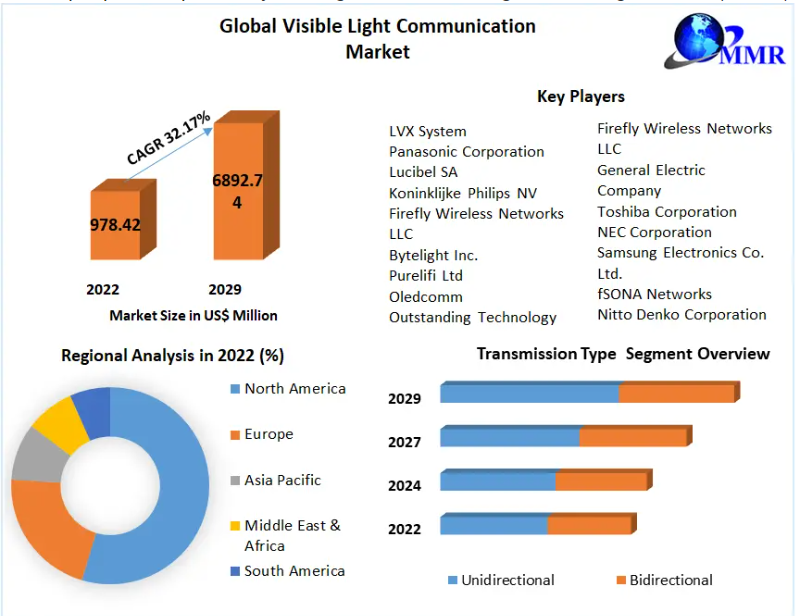
\includegraphics[width=80mm]{visiogeneralVLC.png}
    \caption{visió general de mercat VLC}
    \label{fig:method}
\end{figure}


\begin{figure}[h!]
    \centering
    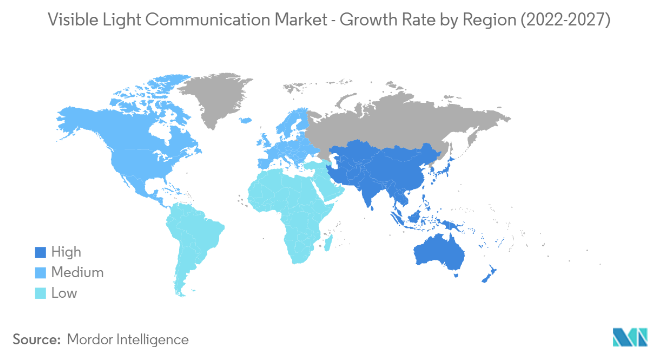
\includegraphics[width=80mm]{futurMundial.png}
    \caption{visió general de mercat VLC}
    \label{fig:method}
\end{figure}


\begin{figure}[h!]
    \centering
    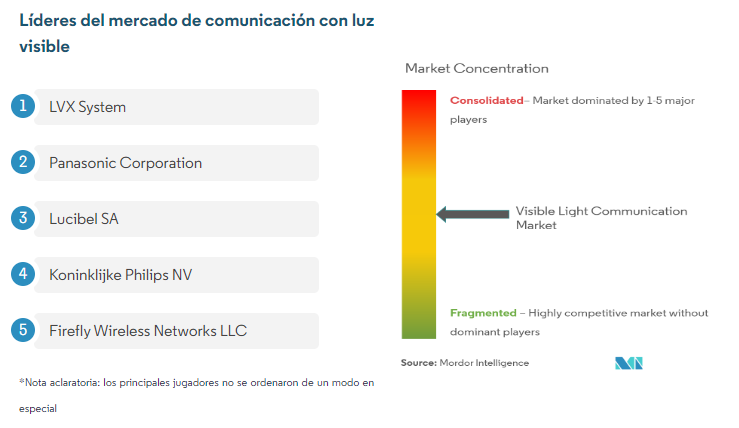
\includegraphics[width=80mm]{liderMercat.png}
    \caption{visió general de mercat VLC}
    \label{fig:method}
\end{figure}


\begin{figure}[h!]
    \centering
    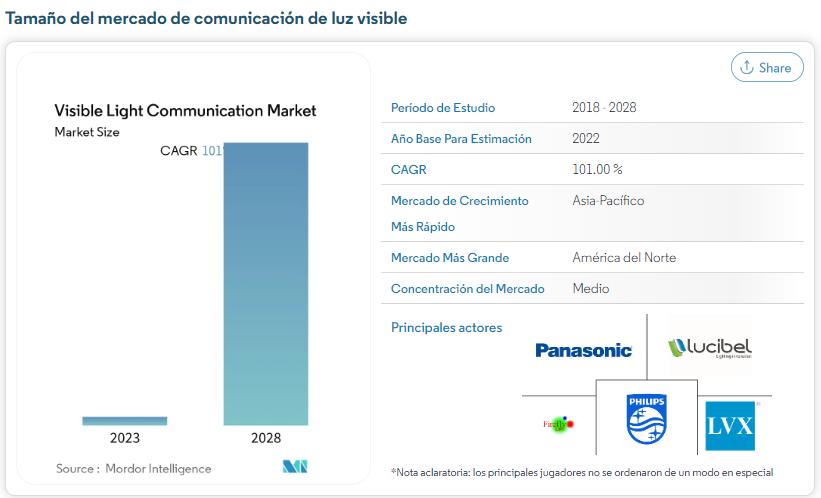
\includegraphics[width=80mm]{tamanyMercat.png}
    \caption{visió general de mercat VLC}
    \label{fig:method}
\end{figure}
